%%%% ijcai23.tex


% These are the instructions for authors for IJCAI-23.

\documentclass{article}
\pdfpagewidth=8.5in
\pdfpageheight=11in

% The file ijcai23.sty is a copy from ijcai22.sty
% The file ijcai22.sty is NOT the same as previous years'
\usepackage{ijcai23}

% Use the postscript times font!
\usepackage{times}
\usepackage{soul}
\usepackage{url}
\usepackage[hidelinks]{hyperref}
\usepackage[utf8]{inputenc}
\usepackage[small]{caption}
\usepackage{graphicx}
\usepackage{amsmath}
\usepackage{amsthm}
\usepackage{booktabs}
\usepackage{algorithm}
\usepackage{algorithmic}
\usepackage[switch]{lineno}
\usepackage{amssymb}

% Comment out this line in the camera-ready submission
% \linenumbers

\urlstyle{same}

% the following package is optional:
%\usepackage{latexsym}

% See https://www.overleaf.com/learn/latex/theorems_and_proofs
% for a nice explanation of how to define new theorems, but keep
% in mind that the amsthm package is already included in this
% template and that you must *not* alter the styling.
\newtheorem{example}{Example}
\newtheorem{theorem}{Theorem}

% Following comment is from ijcai97-submit.tex:
% The preparation of these files was supported by Schlumberger Palo Alto
% Research, AT\&T Bell Laboratories, and Morgan Kaufmann Publishers.
% Shirley Jowell, of Morgan Kaufmann Publishers, and Peter F.
% Patel-Schneider, of AT\&T Bell Laboratories collaborated on their
% preparation.

% These instructions can be modified and used in other conferences as long
% as credit to the authors and supporting agencies is retained, this notice
% is not changed, and further modification or reuse is not restricted.
% Neither Shirley Jowell nor Peter F. Patel-Schneider can be listed as
% contacts for providing assistance without their prior permission.

% To use for other conferences, change references to files and the
% conference appropriate and use other authors, contacts, publishers, and
% organizations.
% Also change the deadline and address for returning papers and the length and
% page charge instructions.
% Put where the files are available in the appropriate places.

% \usepackage{xcolor}
% \newcommand\todo[1]{\textcolor{red}{[#1]}}
% \newcommand\tomek[1]{\textcolor{blue}{TT[#1]}}
% \newcommand\grzesiekk[1]{\textcolor{blue}{GK[#1]}}
% \newcommand\grzesiekr[1]{\textcolor{blue}{GR[#1]}}
% \newcommand\adamp[1]{\textcolor{blue}{AP[#1]}}
% \newcommand\karolinam[1]{\textcolor{blue}{KM[#1]}}
% \newcommand\bartekz[1]{\textcolor{blue}{BZ[#1]}}

\usepackage{subcaption}
\usepackage{pgfplots}
\pgfplotsset{compat=1.18}
\newcommand\smallimg{1.8cm}
\newcommand\smallerimg{1.2cm}
\newcommand{\tabfigure}[2]{\raisebox{-.5\height}{\includegraphics[#1]{#2}}}

\usepackage{array}
\newcolumntype{M}[1]{>{\centering\arraybackslash}m{#1}}


% PDF Info Is REQUIRED.
% Please **do not** include Title and Author information
\pdfinfo{/TemplateVersion (IJCAI.2023.0)}

\title{Active Visual Exploration Based on Attention-Map Entropy}

\author{
% Anonymized authors
Adam Pardyl$^{1,2,3}$\and
Grzegorz Rypeść$^{1,4}$\and
Grzegorz Kurzejamski$^1$\and \\
Bartosz Zieliński$^{1,2,6}$\and
Tomasz Trzciński$^{1,2,4,5}$
\affiliations
$^1$IDEAS NCBR\\
$^2$Jagiellonian University, Faculty of Mathematics and Computer Science\\
$^3$Jagiellonian University, Doctoral School of Exact and Natural Sciences\\
$^4$Warsaw University of Technology\\
$^5$Tooploox\\
$^6$Ardigen
\emails
\{adam.pardyl, grzegorz.rypesc, grzegorz.kurzejamski, bartosz.zielinski, tomasz.trzcinski\}@ideas-ncbr.pl
}

\begin{document}

\maketitle

\begin{abstract}
Active visual exploration addresses the issue of limited sensor capabilities in real-world scenarios, where successive observations are actively chosen based on the environment. To tackle this problem, we introduce a new technique called Attention-Map Entropy (AME). It leverages the internal uncertainty of the transformer-based model to determine the most informative observations. In contrast to existing solutions, it does not require additional loss components, which simplifies the training. Through experiments, which also mimic retina-like sensors, we show that such simplified training significantly improves the performance of reconstruction, segmentation and classification on publicly available datasets.

\end{abstract}

%%%%%%%%%%%%%%%%%%%%%%%%%%%%%%%%%%%%%%%%%%%%%%%%%%%%%%%%%%%%%%%%%%%%%%%%%%%%%%%
\section{Introduction}
\label{sec:intro}

Image-related tasks, such as image reconstruction, segmentation, or scene understanding, usually rely on the assumption of complete and unhindered access to input data~\cite{girdhar2022omnivore}.
 However, in many real-world applications, this assumption is not valid. For example, in the case of an embodied agent, such as a robot, its sensors have often limited registration capabilities, {\it e.g.} restricted field of view, while the environment is constantly changing~\cite{4seasons}. Additionally, the high computational cost of processing large amounts of data and the need for continuous movement further complicates the task of acquiring complete information about the environment. To reason about the whole environment, the agent needs to sample new observations in the most efficient way possible.\footnote{Supplementary material, including the source code, can be found at: \url{https://github.com/apardyl/AME}}

\begin{figure}[t]
\begin{center}
\begin{small}
\begin{sc}
\begin{tabular}{l}
A standard approach based on auxiliary loss func.\\
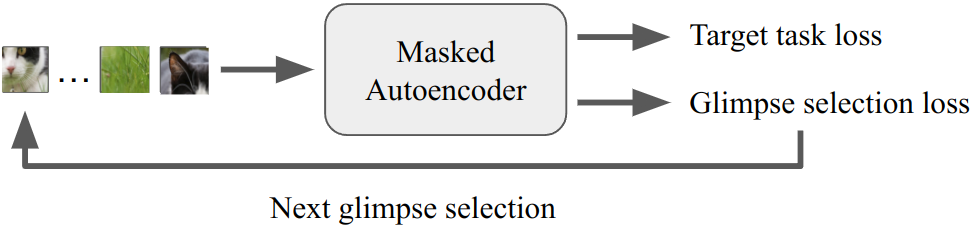
\includegraphics[scale=.23]{fig/teaser/1.png}\\[4pt]
\hline \\[\dimexpr-\normalbaselineskip+4pt]
Our approach based on internal MAE uncertainty\\
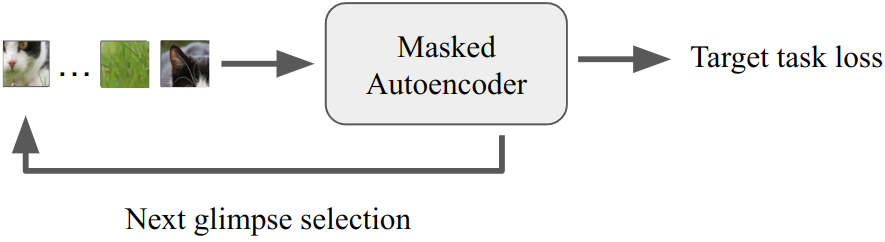
\includegraphics[scale=.23]{fig/teaser/2.png}
\end{tabular}
\end{sc}
\end{small}
\end{center}
\vskip -0.1in
\caption{\textbf{Attention-Map Entropy (AME):} Our approach chooses the most informative observations by reusing the internal uncertainty coded in the attention maps. In contrast to existing methods, it does not require any auxiliary loss functions dedicated to active exploration. Therefore, the training concentrates on the target task loss, not on an auxiliary loss, which improves overall performance.}
\label{fig:teaser}
\end{figure}

Previous works in the field of embodied visual exploration have leveraged various sampling strategies to improve results on localization and mapping tasks \cite{Ramakrishnan2021AnEO}. Many of these methods use reinforcement learning \cite{ramakrishnan2018rl3} and multiple custom uncertainty measures \cite{Ramakrishnan2021AnEO}, but they can be complex and difficult to train. To overcome this issue, \cite{seifi2019wheretolooknext} introduced a streamlined architecture based on convolutional networks. They also simplified the setup for selecting image patches within a frame, referred to as glimpses, from 360$^{\circ}$ images in reconstruction tasks. The idea was further extended for segmentation task \cite{seifi2020segment}. %, bringing additional local and global extraction modules.
In both scenarios, the choice of where to sample next was determined by using separate heads that output probability maps indicating the location of the next glimpse. In \cite{seifi2021glimpse}, they proposed a method of using attention pooling layers in a task-driven architecture to generate probability maps. However, this complex solution consisted of five separate training streams, each with its own optimization goals and a contrastive learning approach.

Furthermore, these existing methods involve separate training for the main task and the sampling decision strategy, which increases computational overhead of the entire system. \cite{Jha2023WACV} addresses this limitation by using a~transformer-based auto-encoder with a glimpse selection neural head. % and abandoning the global memory-map approach.
Nevertheless, all previous works rely on a dual approach to the active exploration problem. One target function is optimized to improve the quality of the main task, while another one is aimed at training the sampling decision strategy. This introduces unnecessary complexity of the model, increases the number of neural network components and yields more memory-heavy solutions.

In this paper, we address these complexity issues by introducing a transformer-based active vision method that leverages internal model uncertainty for next glimpse selection. Inspired by~\cite{Aloimonos1988}, we train our method to explore a scene by gathering partial observations about it sequentially without incorporating any separate sampling decision module. % or decision strategy-related training elements. 
Contrary to the recent solution \cite{Jha2023WACV}, we use attention values trained inherently within the transformer-based decoder to generate decision-making priors, which provides superior performance over both random sampling and state-of-the-art solutions.

Our strategy for glimpse selection is based on the entropy of the transformer's attention maps and thus needs suitable architecture for the main task. Similarly to \cite{Jha2023WACV}, we base our network on masked autoencoder (MAE \cite{he2022masked}) to efficiently deal with the problem of partially available input.% and mitigate the need for global-level memory maps. 

We evaluate our approach using common benchmarks and relevant competing methods for reconstruction, classification, and segmentation tasks. Furthermore, we test our solution using both full-resolution patches, and retina-like glimpses \cite{sandini2003retina}, publishing for the first time the empirical results for the latter data when coupled with transformer-based architectures.

We can summarize our contributions as follows:
\begin{itemize}
    \item We present a new approach to glimpse selection in active visual exploration that leverages the internal transformer uncertainty stored in attention maps, eliminating the need for additional loss components.
    \item We validate our method with multiple patch configurations, including retina-like glimpses mimicking retina-like sensors. %, and apply them to transformer-based architectures.
    \item We thoroughly evaluate our solution on various visual tasks, demonstrating its superiority over the existing methods and various selection alternatives.
\end{itemize}

%%%%%%%%%%%%%%%%%%%%%%%%%%%%%%%%%%%%%%%%%%%%%%%%%%%%%%%%%%%%%%%%%%%%%%%%%%%%%%%
\section{Related Works}

\paragraph{Missing data.}
Our tasks are strictly connected with a missing data problem addressed by various research works. Some of them, like~\cite{smieja2018processing}, concentrate on fully connected networks where the missing data can be estimated with input data distribution. Other approaches concentrate on visual inpainting using adversarial and reconstruction loss~\cite{pathak2016context}. \cite{li2022mat} address the inpainting problem by using transformer architecture with a local masking scheme in attention layers, resulting in computation savings. \cite{naseer2021visionTransformers} analyze well-known CNNs and claims they reach as low as 20\% accuracy in ImageNet evaluation after masking only 20\% of the image. Adequate progress in this field was made in Masked Auto-encoders (MAE) \cite{he2022masked} where authors use arbitrarily chosen masked parts of the input data to enrich visual features and regularize the training. Our method builds upon the MAE architecture, proven to achieve significant results in partially-masked image reconstruction.

\paragraph{Active visual exploration.} 
Many works discuss simultaneous localization and mapping (SLAM) challenges in the context of active exploration \cite{Ramakrishnan2021AnEO}. \cite{samrudhdhi2021vae1} use the variational auto-encoder to hallucinate multiple hypotheses of the unseen parts of the image and infer uncertainty scores, which are further used to select the next glimpse parameters. Authors of~\cite{seifi2021glimpse,seifi2020segment,seifi2019wheretolooknext} presented various solutions for active visual exploration, notably using CNN-based attention maps for glimpse selection and contrastive learning for global feature maps training. \cite{Jha2023WACV} introduces MAE-based~\cite{he2022masked} autoencoder with additional glimpse decision neural network to solve image reconstruction tasks. Results of these works have been reported in reconstruction, segmentation, and classification tasks, giving suitable baselines for our research. Our method solves the active visual exploration problem, but in contrast to the existing method, it uses auto-encoder internal, task-driven uncertainty to select successive glimpses.

\paragraph{Glimpse Selection.} 
As opposed to solutions imposed by SLAM tasks, many researchers present glimpse selection problems in other contexts. For example, \cite{chai2019rl2} adopts a deep reinforcement learning approach based on attention mechanisms to choose the best patch from consecutive video frames, yielding significant computational savings. \cite{jayaraman2017rl1} use uncertainty measures with reinforcement learning to estimate the following observations' parameters for a single 3D object analysis setup. \cite{rangrej2022consistency} introduces classification transformer architecture with an actor-critic module with an uncertainty estimator used for patch sampling. In our work, we actively search for successive glimpses defining the next patch sample using the entropy of the transformer attention maps. In opposition to \cite{rangrej2022consistency} or \cite{Jha2023WACV}, we do not need an additional neural network to make a glimpse decision. We also use no additional losses except those related to the target task.

%%%%%%%%%%%%%%%%%%%%%%%%%%%%%%%%%%%%%%%%%%%%%%%%%%%%%%%%%%%%%%%%%%%%%%%%%%%%%%%
\section{Method}

\begin{figure}[t]
\centerline{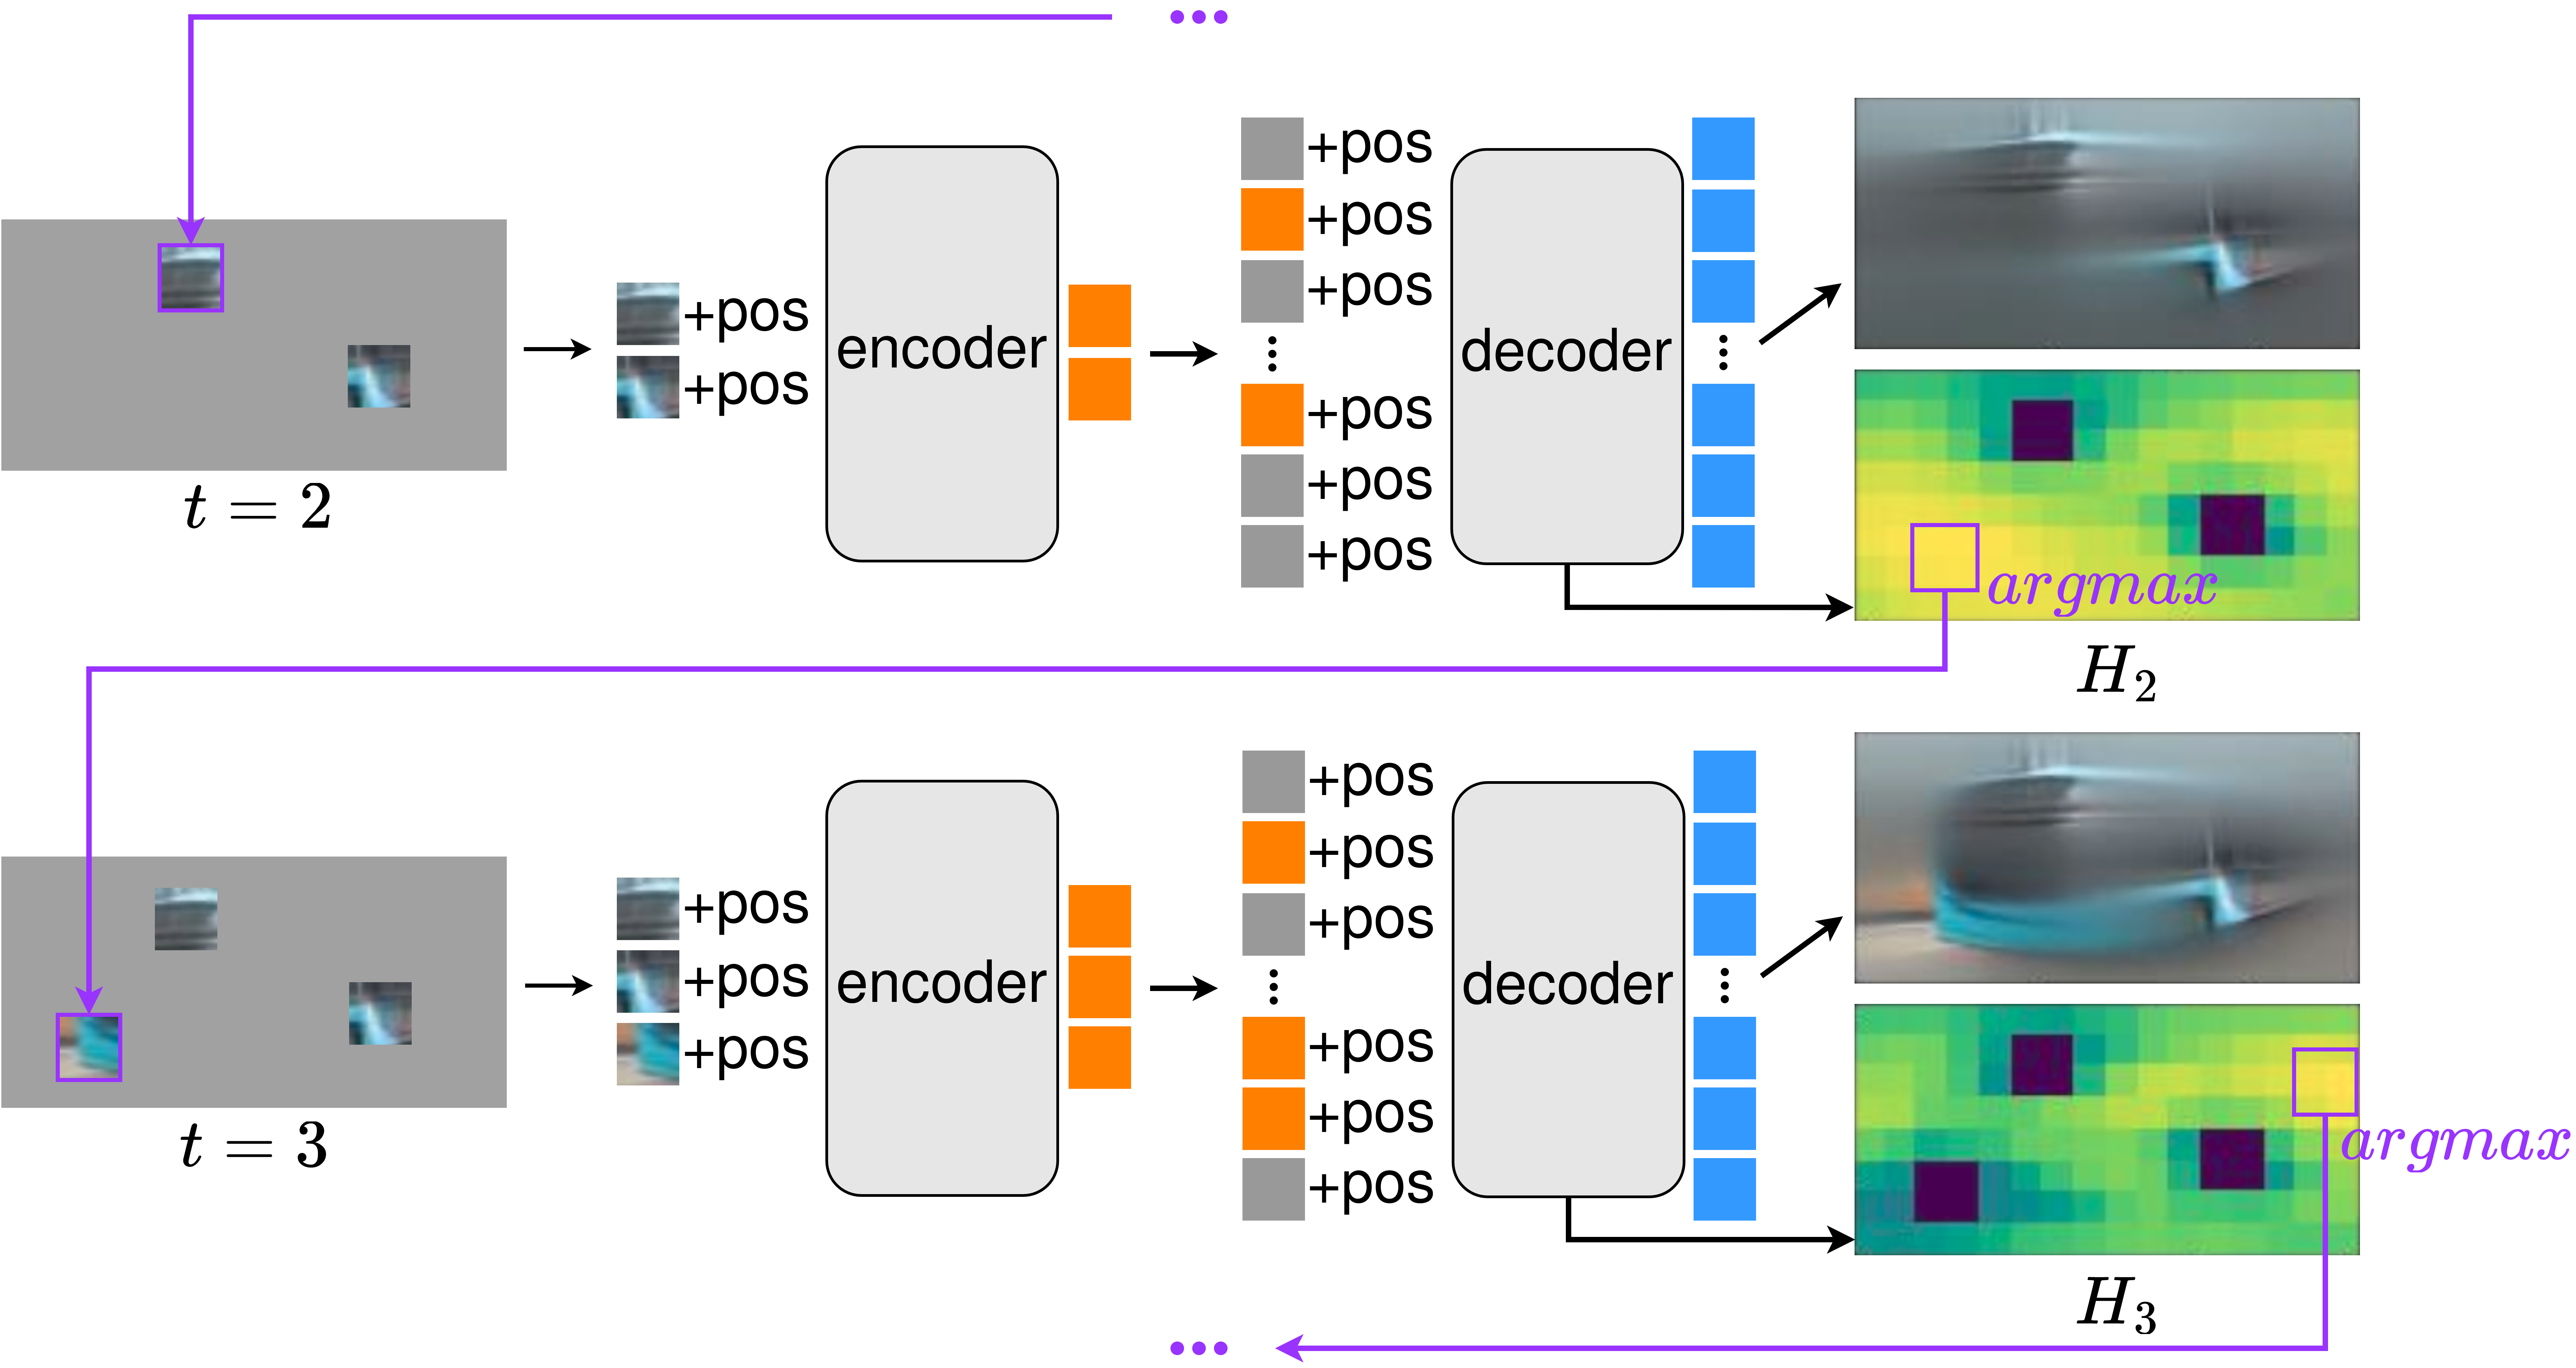
\includegraphics[width=\linewidth]{architecture.png}}
\caption{\textbf{Architecture for reconstruction:} The agent observed two patches of the image, which are processed by the encoder to produce their feature representations (orange rectangles). These outputs are combined with the masked patches (shown as gray rectangles) and passed through the decoder. The decoder reconstructs the missing image patches. Additionally, our method generates the entropy map for one of the decoder's multi-head self-attention layers and uses it to select the location of the third glimpse. The process repeats till we reach the assumed number of glimpses.}
\label{fig_overview}
\end{figure}

The fundamental idea of our approach is to leverage the internal uncertainty of the transformer-based autoencoder to select the most informative glimpses to be explored. Therefore, instead of using an additional loss function for glimpse selection, we propose a new method that obtains successive glimpses by analyzing the entropy of attention maps. This way, we can select the patch that has the highest entropy and confuses our model the most,  %the most confusing patches more directly, 
which improves the convergence of our method and reduces its complexity compared to the existing methods. 

As presented in Figure \ref{fig_overview}, our approach is based on a masked autoencoder with $T$ run-times. In the beginning, we run it for one glimpse, and at step $t < T$, there are $t$ known glimpses. To select the $t+1$ glimpse, we pass $t$ glimpses selected so far through the masked autoencoder and calculate entropy for its attention maps. The masked patch with the highest entropy is chosen as the next glimpse. The network produces the final output for the target task ({\it e.g.} a reconstructed image for a reconstruction task) for $t = T$. This selection process is described in Section~\ref{glimpse-selection}. Moreover, in Section~\ref{sec:mae} and Section~\ref{sec:finalTask}, we describe the transformer-based autoencoder and the adjustments of its architecture to various target tasks.

\subsection{Transformer-based Masked Autoencoder}
\label{sec:mae}

Our approach employs a transformer-based Masked Autoencoder (MAE) network, as outlined in \cite{he2022masked}, which includes an encoder and a decoder.

The encoder is a modified version of the Vision Transformer (ViT)~\cite{dosovitskiy2020image}. As an input at a step $t$, it obtains a sequence of patches $p_1, p_2, ..., p_t: \forall_i p_i\in \mathbb{R}^{P^2 \times C}$ observed so far, where $P$ is the patch size, and $C$ is the number of input image channels. The patches are projected into $E$-dimensional embeddings using a linear layer and summed with positional embeddings. Then, they are processed through transformer blocks together with a learnable \textsc{cls} token, resulting in $t$ latent embeddings of dimension $D$. Because the number of visible patches may vary between images in a batch, we employ transformer blocks that allow pad tokens similar to those proposed in~\cite{vaswani2017attention}.

The decoder is a transformer with a linear head that operates on $t$ latent embeddings generated by the encoder and the coded positions of the $\frac{HW}{P^2} - t$ remaining patches, where $H$ and $W$ represent the height and width of the input image. The concatenated embeddings of dimension $D$ are positionally encoded and processed through transformer blocks. The last part of the decoder is a linear layer with dimensions varies depending on the task (see Section~\ref{sec:finalTask}).

\subsection{Glimpse Selection}
\label{glimpse-selection}

\begin{figure}[t]
\centerline{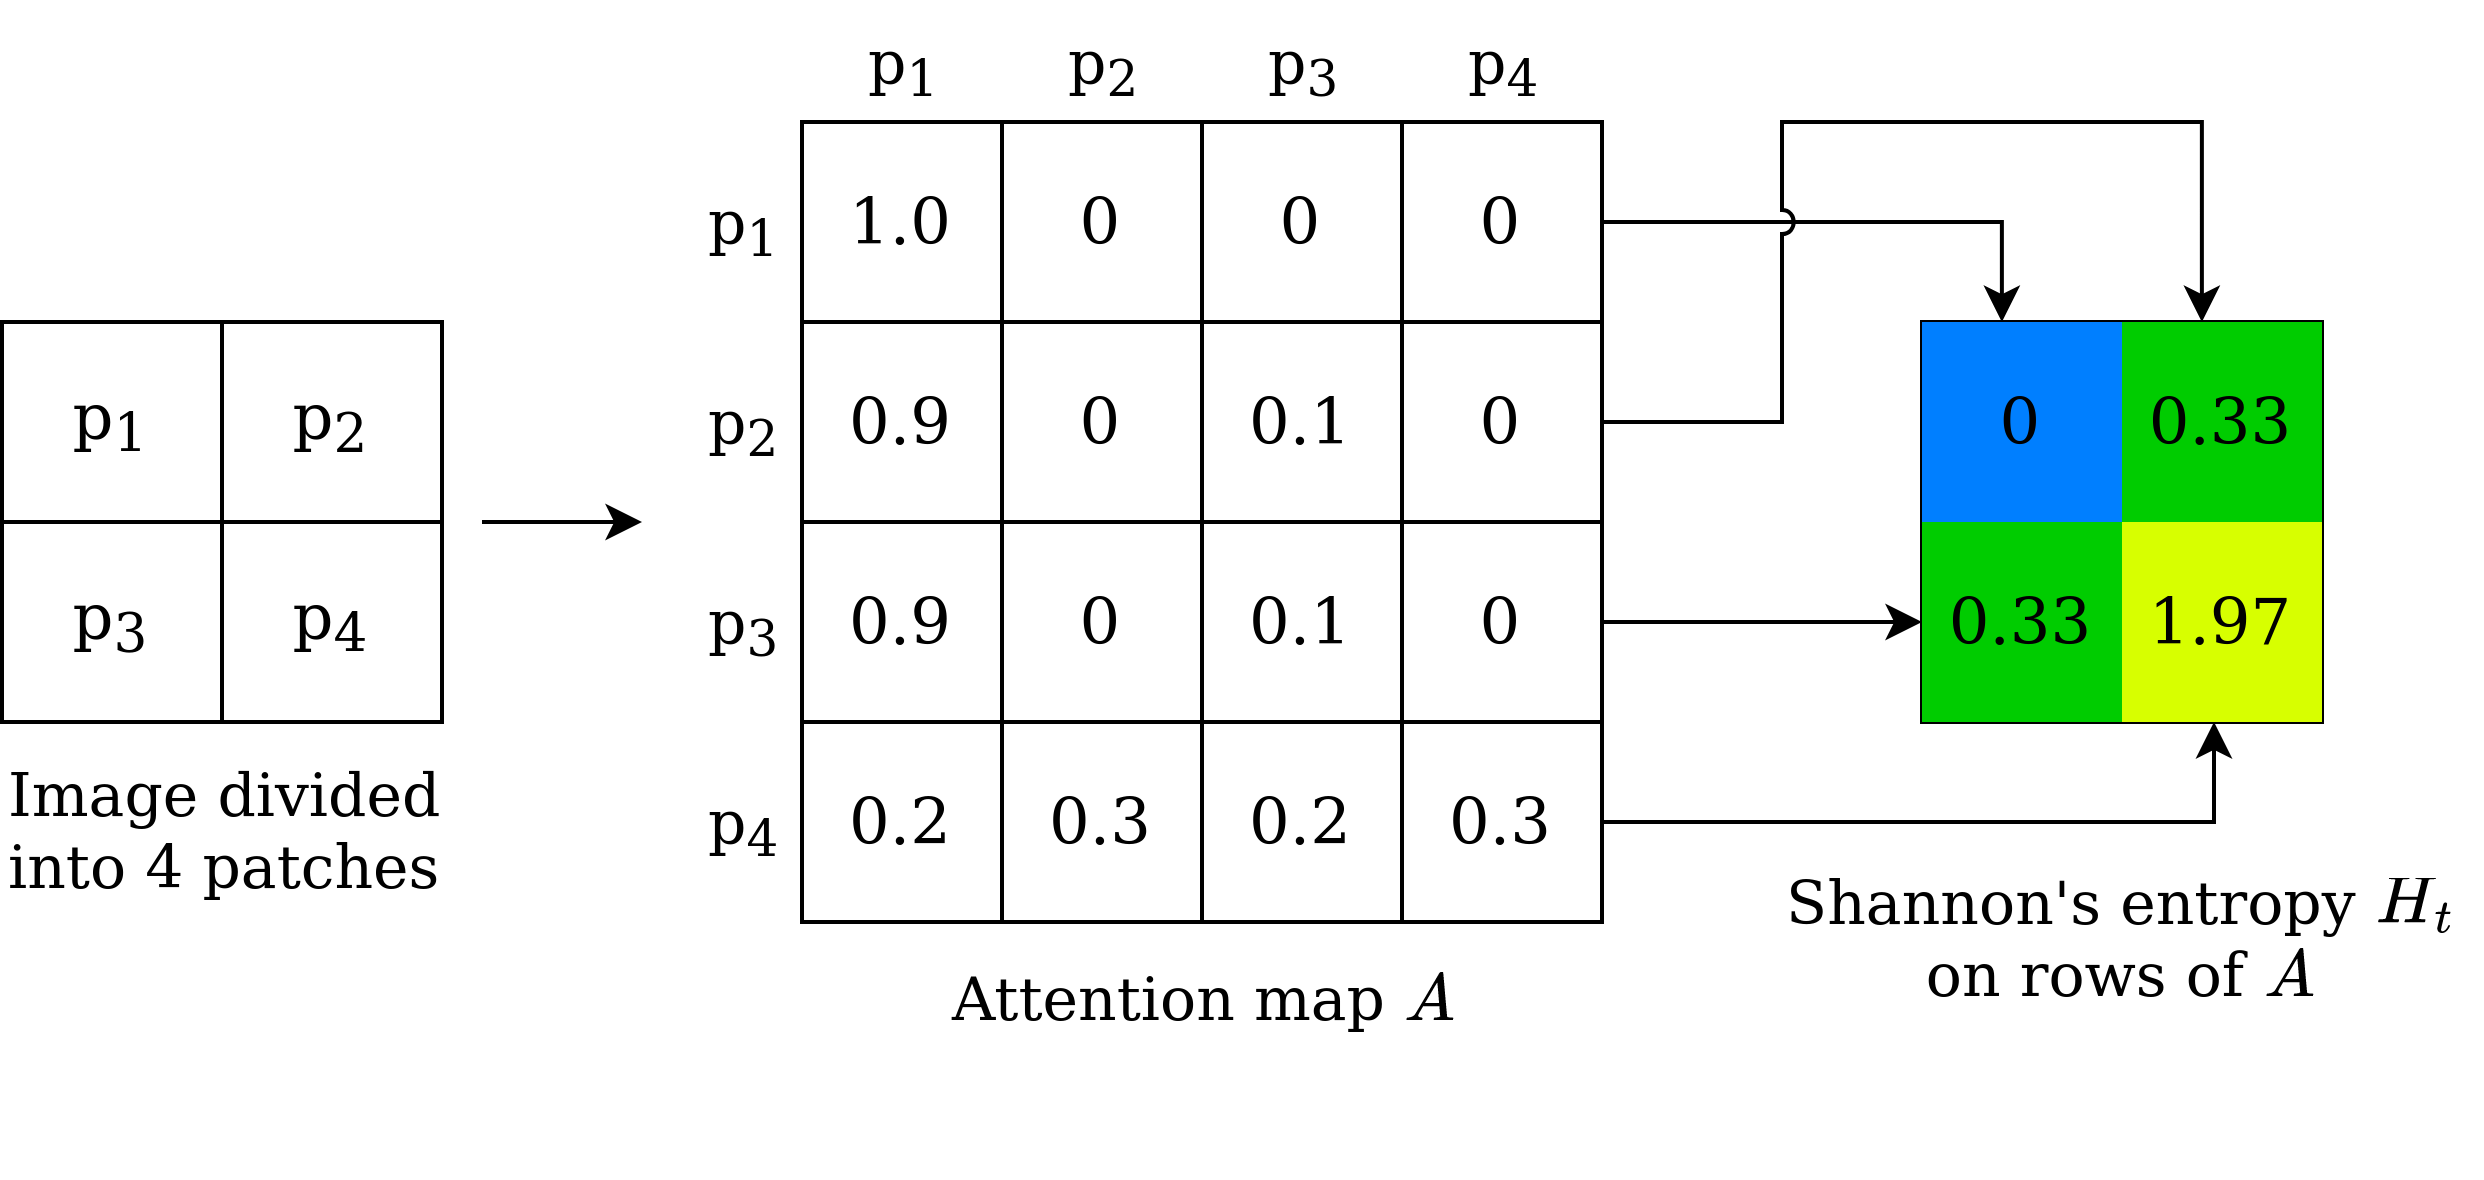
\includegraphics[width=\linewidth]{fig/shannon.png}}
\caption{\textbf{Entropy map:} To explain the idea of the entropy map based on attention in the transformer layer, let us consider an image divided into four patches ($2 \times 2$) on the left. Its attention map will be a $4 \times 4$ matrix, where each row represents the attention weights used to calculate the output in the next transformer layer for a corresponding patch. Calculating Shannon's entropy for each row will result in a $2 \times 2$ entropy map. The patch with the highest entropy value is selected as the next glimpse.}
\label{fig:selection}
\end{figure}

To explore the internal uncertainty of transformer-based models, we analyze the entropy of the attention map~\cite{vaswani2017attention}, as presented in Figure~\ref{fig:selection}. For this purpose, we start with calculating attention map $A \in \mathbb{R}^{t \times t}$ for patches $p_1, p_2, ..., p_t$ obtained so far as
\begin{equation}
A = \textrm{softmax}(K K^T / \sqrt{d_k}),
\end{equation}
where $K \in \mathbb{R}^{t \times D}$ is a matrix that packs together all embeddings of patches from one of the decoder's layers.
%
The successive rows of $A$ contain weights used to calculate a weighted average of the patches outputs. Therefore, to obtain the output for patch $i$, we sum the values of all patches weighted with $A[i]$ ($i$-th row of $A$).

However, we can observe that the entropy of $A$ rows significantly differs, and it can be used to select an adequate candidate for the next glimpse. To explain how, let us consider patches $2$ and $4$ from Figure~\ref{fig:selection} with $A[2]=[0.9, 0, 0.1, 0]$ and $A[4]=[0.2, 0.3, 0.3, 0.2]$. While the $2$nd patch output is obtained based mostly on the value of the $1$st patch, the $4$th patch output is obtained based on all other patches. Hence, the model is confident about the $2$nd patch but is uncertain about patch $4$. Therefore, the latter is a better candidate for the next glimpse, as it needs to be explored.

To formalize this idea, let us also recall that transformers use multi-head attention, which computes multiple attention maps, each for embeddings obtained with different linear projections. Therefore, assuming that $A_{h,t}$ denotes the attention map of $h$th head in step $t$, the entropy map for a given multi-head self-attention layer is calculated as
\begin{equation}
H_t = \sum_h H(A_{h,t}[i]),
\label{eq:h_t}
\end{equation}
where $H$ is the Shannon entropy. Then, we replace entropy values for known patches to $0$ to omit them in the further selection process, and we choose the patch with the maximal value of $H_t$ as the next glimpse
\begin{equation}
i^* = \textrm{argmax}_{i=1,\dots,d_{model}} H_t[i].
\end{equation}

\begin{figure*}[t]
\begin{center}
\begin{small}
\begin{sc}
\begin{tabular}{r@{\hskip2pt}c@{\hskip2pt}c@{\hskip2pt}c@{\hskip2pt}c@{\hskip2pt}c@{\hskip2pt}c@{\hskip2pt}c@{\hskip2pt}c@{\hskip2pt}|@{\hskip2pt}M{\smallimg}}
a) & 1 & 2 & 3 & 4 & 5 & 6 & 7 & 8 & \\[3pt]
b) &\tabfigure{width=\smallimg}{fig/steps/1_masked.jpg} & \tabfigure{width=\smallimg}{fig/steps/2_masked.jpg} & \tabfigure{width=\smallimg}{fig/steps/3_masked.jpg} & \tabfigure{width=\smallimg}{fig/steps/4_masked.jpg} & \tabfigure{width=\smallimg}{fig/steps/5_masked.jpg} & \tabfigure{width=\smallimg}{fig/steps/6_masked.jpg} & \tabfigure{width=\smallimg}{fig/steps/7_masked.jpg} & \tabfigure{width=\smallimg}{fig/steps/8_masked.jpg} & Ground truth\\[13pt]
c) &\tabfigure{width=\smallimg}{fig/steps/1_out.jpg} & \tabfigure{width=\smallimg}{fig/steps/2_out.jpg} & \tabfigure{width=\smallimg}{fig/steps/3_out.jpg} & \tabfigure{width=\smallimg}{fig/steps/4_out.jpg} & \tabfigure{width=\smallimg}{fig/steps/5_out.jpg} & \tabfigure{width=\smallimg}{fig/steps/6_out.jpg} & \tabfigure{width=\smallimg}{fig/steps/7_out.jpg} & \tabfigure{width=\smallimg}{fig/steps/8_out.jpg}& {\raisebox{-.28\height}{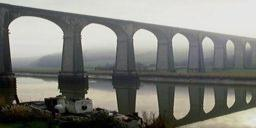
\includegraphics[width=\smallimg]{fig/steps/0_input.jpg}}}  \\[13pt]
d) &\tabfigure{width=\smallimg}{fig/steps/1_entropy.jpg} & \tabfigure{width=\smallimg}{fig/steps/2_entropy.jpg} & \tabfigure{width=\smallimg}{fig/steps/3_entropy.jpg} & \tabfigure{width=\smallimg}{fig/steps/4_entropy.jpg} & \tabfigure{width=\smallimg}{fig/steps/5_entropy.jpg} & \tabfigure{width=\smallimg}{fig/steps/6_entropy.jpg} & \tabfigure{width=\smallimg}{fig/steps/7_entropy.jpg} &&
\end{tabular}
\end{sc}
\end{small}
\end{center}
\vskip -0.1in
\caption{\textbf{Glimpse-based reconstruction step-by-step:} The figure shows a glimpse selection process based on AME for $8\times32^2$ glimpses for a sample $256\times128$ image. The rows correspond to \textsc{a)} step number, \textsc{b)} model input (glimpses), \textsc{c)} model prediction given, \textsc{d)} decoder attention entropy (known areas are explicitly set to zero). The algorithm explores the image in places where the reconstruction result is blurry.}
\label{fig:steps}
\end{figure*}


\subsection{Differences Caused by Final Task}
\label{sec:finalTask}

For the reconstruction and segmentation tasks, the last layer of the decoder returns a representation of dimension $C' \times P^2$ for each processed patch, where $C'$ is the number of input image channels for reconstruction and the number of segmented classes for segmentation. In this case, the output for the \textsc{cls} token is omitted. For the classification task, we add an auxiliary classification head, which takes the \textsc{cls} token from the encoder as input to classify the image.

%%%%%%%%%%%%%%%%%%%%%%%%%%%%%%%%%%%%%%%%%%%%%%%%%%%%%%%%%%%%%%%%%%%%%%%%%%%%%%%
\section{Experimental Setup}
\label{sec:setup}

\subsection{General considerations}

\paragraph{Architecture.} In all our experiments, we use 24 transformer blocks in the encoder, with an embedding size of 1024 (the same parameters as the ViT-L architecture \cite{dosovitskiy2020image}), and 8 decoder blocks with an embedding size of 512. We use the AdamW optimization algorithm \cite{loshchilov2018decoupled} with a weight decay value of 0 for reconstruction and $10^{-4}$ for other tasks. The learning rate is first linearly brought up to $10^{-4}$ for the first 10 training epochs, then decayed with the half-cycle cosine rate to $10^{-8}$ for the rest of the training. We train the model for $75$ epochs with early stopping. We augment the training data with random scaling, cropping, and horizontal flipping. Then we resize the image to the required size. Unless otherwise specified, we initialize the model with MAE \cite{he2022masked} weights trained on the ImageNet-1K \cite{deng2009imagenet} dataset. For $256\times128$ images, we also fine-tune those MAE weights on the target resolution using the MS COCO dataset \cite{lin2014microsoft} using the original MAE implementation. For glimpse selection, we extract the attention map from the last decoder block. The first glimpse is selected by the entropy mechanism run with mask tokens only (zero known patches).

\paragraph{Datasets.} We evaluate our method on 3 different vision datasets. The largest one, MS COCO dataset (Common Objects in Context; 2014 split version)~\cite{lin2014microsoft}, consists of ~83K train images and ~41K validation images. The second one, ADE20K~\cite{zhou2017scene} dataset, consists of ~26K training and 2k validation images, containing 150 classes for the semantic segmentation task. The smallest one is SUN360~\cite{song2015sun} dataset with approximately 8K $360^{\circ}$ panoramic images, unevenly split between 26 classes for the multi-class classification task. As the last dataset does not have a predetermined train-test split, we use a $9:1$ train-test split based on an index provided by authors of \cite{seifi2021glimpse}.

\paragraph{Glimpse regimes and baselines.} We perform the experiments in two different glimpse regimes associated with two sets of state-of-the-art baselines.

First, we compare our method against fully convolutional approaches: Attend and segment~\cite{seifi2020segment} and Glimpse, attend and explore~\cite{seifi2021glimpse}. Both methods use three-level retina-like glimpses, simulating the use of retina-like sensors introduced in~\cite{sandini2003retina}. In this setup, an image is resized to $256\times128$ pixels, and the algorithm extracts 8 retinal glimpses of size 48x48 pixels. This corresponds to extracting 18.75\% of pixels (accounting for retinal down-scaling) and 56.26\% of the image area explored. As glimpses consist of multiple ViT patches, during the glimpse selection process, we average the glimpse selection map from Equation~\ref{eq:h_t} over the size of a glimpse.

Secondly, we compare it to a transformer-based method called SimGlim~\cite{Jha2023WACV}. In this scenario, an image is resized to $224 \times 224$ pixels, and we extract 37 regular (non-retinal) glimpses of size 16x16 pixels (one ViT patch~\cite{dosovitskiy2020image}). As a result, 18.75\% of pixels are extracted, covering 18.75\% of the image area.

The results of baseline methods (including visualizations) are copied from the original papers because we could not reproduce them due to incomplete or missing code.

We also conducted ablation experiments using two naive sampling methods. The first method is random sampling, which has the potential for overlap of glimpses. The second method samples glimpses from a fixed, non-overlapping checkerboard pattern~\cite{he2022masked}.

\subsection{Tasks}

\begin{table*}[t]
\begin{center}
\begin{small}
\begin{sc}
\begin{tabular}{lrrrllrr}
\toprule
Method & SUN360 & ADE20k & MS COCO & Image res. & Glimpse regime & Pixel \% & Area \% \\
\midrule
AttSeg & 37.6 & 36.6 & 41.8 & $128 \times 256$ & $8 \times 48^2$ (retinal) & 18.75 & 56.25 \\
GlAtEx & 33.8 & 41.9 & 40.3 & $128 \times 256$ & $8 \times 48^2$ (retinal) & 18.75 & 56.25 \\
Ours (retinal) & \textbf{23.6} & \textbf{23.8} & \textbf{25.2} & $128 \times 256$ & $8 \times 48^2$ (retinal) & 18.75 & 56.25\\
\midrule
Ours (non-retinal) & 37.9 & 40.7 & 43.2 & $128 \times 256$ & $8 \times 16^2$ (non ret.) & 6.25 & 6.25\\
Ours (non-retinal) & 29.8 & 30.8 & 32.5 & $128 \times 256$ & $8 \times 32^2$ (non ret.) & 25.00 & 25.00\\
Ours (non-retinal) & \textbf{20,1} & \textbf{20.6} & \textbf{22.1} & $128 \times 256$ & $8 \times 48^2$ (non ret.) & 56.25 & 56.25 \\
\midrule
SimGlim (detached) & 26.2 & 27.2 & 29.8 & $224 \times 224$ & $37 \times 16^2$ (non ret.) & 18.75 & 18.75\\
SimGlim (end-to-end) & 28.0 & 28.8 & 31.3 & $224 \times 224$ & $37 \times 16^2$ (non ret.) & 18.75 & 18.75 \\
Ours (non-retinal) & \textbf{23.4} & \textbf{26.2} & \textbf{28.6} & $224 \times 224$ & $37 \times 16^2$ (non ret.) & 18.75 & 18.75 \\
\bottomrule
\end{tabular}
\end{sc}
\end{small}
\end{center}
\vskip -0.1in
\caption{\textbf{Reconstruction results:} Comparison of our model in reconstruction task against AttSeg~\protect\cite{seifi2020segment}, GlAtEx~\protect\cite{seifi2021glimpse} and SimGlim~\protect\cite{Jha2023WACV} on SUN360, ADE20K and MS COCO datasets. The metric used is a root mean square error (RMSE; lower is better). For each experiment, we provide a training and evaluation regime defined by a number of glimpses of a specific resolution. Pixel \% and area \% denote respectively: the percentage of image pixels known to the model and the percentage of image area seen by the model. Differences in both measures occur when dealing with retina-like glimpses, which have lower pixel counts by design. Our method outperforms competitive solutions in all configurations.}
\label{tab:reconstruction}
\end{table*}

\begin{figure}[t]
\begin{center}
\begin{small}
\begin{sc}
\begin{tabular}{c@{\hskip2pt}c@{\hskip2pt}c@{\hskip2pt}c}
Input&Ours&GlAtEx&AttSeg\\
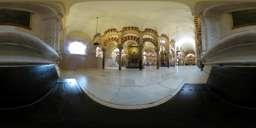
\includegraphics[width=\smallimg]{fig/sun360/1/gt.jpg}&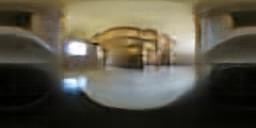
\includegraphics[width=\smallimg]{fig/sun360/1/ours.jpg}&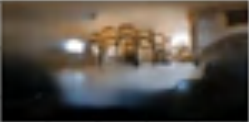
\includegraphics[width=\smallimg]{fig/sun360/1/glatex.png}&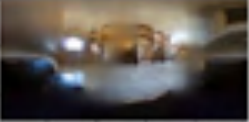
\includegraphics[width=\smallimg]{fig/sun360/1/atseg.png}\\

\includegraphics[width=\smallimg]{fig/sun360/2/gt.jpg}&
\includegraphics[width=\smallimg]{fig/sun360/2/ours.jpg}&
\includegraphics[width=\smallimg]{fig/sun360/2/glatex.png}&
\includegraphics[width=\smallimg]{fig/sun360/2/atseg.png}\\

\includegraphics[width=\smallimg]{fig/sun360/3/gt.jpg}&
\includegraphics[width=\smallimg]{fig/sun360/3/ours.jpg}&
\includegraphics[width=\smallimg]{fig/sun360/3/glatex.png}&
\includegraphics[width=\smallimg]{fig/sun360/3/atseg.png}\\

\includegraphics[width=\smallimg]{fig/sun360/5/gt.jpg}&
\includegraphics[width=\smallimg]{fig/sun360/5/ours.jpg}&
\includegraphics[width=\smallimg]{fig/sun360/5/glatex.png}&
\includegraphics[width=\smallimg]{fig/sun360/5/atseg.png}\\
\end{tabular}
\end{sc}
\end{small}
\end{center}
\vskip -0.1in
\caption{\textbf{Reconstruction quality for SUN360:} Reconstruction results of our method compared with AttSeg~\protect\cite{seifi2020segment} and GlAtEx~\protect\cite{seifi2021glimpse} on the SUN360 dataset. Reconstructions done with our method are visibly better than the competition.}
\label{fig:qualiative-retinal}
\end{figure}

\begin{figure}[t]
\begin{center}
\begin{small}
\begin{sc}
\begin{tabular}{c@{\hskip2pt}c@{\hskip2pt}c|c@{\hskip2pt}c@{\hskip2pt}c}
Input&Ours&SimGlim&Input&Ours&SimGlim\\

\includegraphics[width=\smallerimg]{fig/ade/3/gt.jpg}&
\includegraphics[width=\smallerimg]{fig/ade/3/ours.jpg}&
\includegraphics[width=\smallerimg]{fig/ade/3/simglim.png}&

\includegraphics[width=\smallerimg]{fig/ade/2/gt.jpg}&
\includegraphics[width=\smallerimg]{fig/ade/2/ours.jpg}&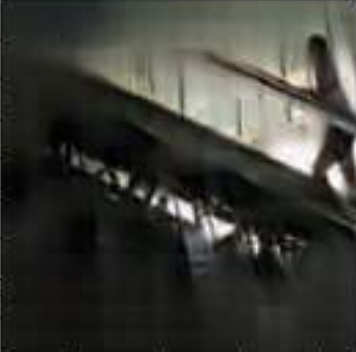
\includegraphics[width=\smallerimg]{fig/ade/2/simglim.png}\\

\includegraphics[width=\smallerimg]{fig/ade/4/gt.jpg}&
\includegraphics[width=\smallerimg]{fig/ade/4/ours.jpg}&
\includegraphics[width=\smallerimg]{fig/ade/4/simglim.png}&

\includegraphics[width=\smallerimg]{fig/ade/5/gt.jpg}&
\includegraphics[width=\smallerimg]{fig/ade/5/ours.jpg}&
\includegraphics[width=\smallerimg]{fig/ade/5/simglim.png}\\
\end{tabular}
\end{sc}
\end{small}
\end{center}
\vskip -0.1in
\caption{\textbf{Reconstruction quality for ADE20K:} Figure shows difference in reconstruction quality against SimGlim~\protect\cite{Jha2023WACV} on the ADE20K dataset. SimGlim reconstructs a single object slightly better, but our method recovers more objects in the scene.}
\label{fig:qualiative-non-retinal}
\end{figure}

\paragraph{Reconstruction.} The reconstruction task involves recreating the ground-truth image with a limited number of glimpses. We evaluate our method on the MS COCO, ADE20K, and SUN360 datasets. The reconstruction quality is measured using the Root Mean Squared Error (RMSE), also used as a loss function.

\paragraph{Classification.} We evaluate our model in the multi-class classification task on the SUN360 dataset using a limited number of glimpses. We use accuracy as a metric and cross entropy as a loss function. We evaluate our model in two training regimes: a) training the entire model for classification (\textit{train-all}) and b) training only the classification head-on features generated by a model trained on the reconstruction task (\textit{head-only}).
The classification head consists of linear layers: one in the \textit{train-all} scenario or two separated by a GELU activation layer for the \textit{head-only} scenario. For the \textit{train-all} scenario, we do a weighted sum of the classification loss (cross-entropy) and a loss of the decoder (required for the glimpse selection mechanism).

\paragraph{Segmentation.} The goal of the segmentation task is to classify each pixel of the input image. Our method is tested on the ADE20K dataset. The mean Pixel Accuracy (mPA; averaged over classes), Pixel Accuracy (PA; averaged over all pixels), and Intersection over Union (IoU) are used as a metric, and the pixel-wise cross-entropy is used as a loss function. We initialize the transformer weights in two ways: using MAE or SETR (trained on ADE20k) weights as the source of encoder weights. In both cases, the decoder is initialized randomly.

%%%%%%%%%%%%%%%%%%%%%%%%%%%%%%%%%%%%%%%%%%%%%%%%%%%%%%%%%%%%%%%%%%%%%%%%%%%%%%%
\section{Results}

To illustrate how the glimpse selection process works step by step, we present it in Figure \ref{fig:steps} on a sample image from the ADE20K dataset. As can be seen, with each glimpse, not only the glimpse neighborhood but the entire output image becomes clearer because the transformer gains a better understanding of the scene.

\subsection{Reconstruction}


In our study, we demonstrate superior performance in the retina-like glimpse setup for all datasets examined. Supporting results are presented in the top part of Table \ref{tab:reconstruction}. Additionally, as shown in Figure \ref{fig:qualiative-retinal}, the reconstructions produced by our method are of higher quality, with visibly increased clarity and sharpness.

We also conduct tests without retina degradation of patches and show that using non-retinal glimpses improved results by over 10\% of all scores. Moreover, our tests with smaller non-retinal patch sizes show that we still achieved better RMSE scores using less than half the area. In this experiment, we use eight patches in a 32x32 resolution, using 25\% of the area compared to 56.25\% in baseline, as seen in the middle part of Table \ref{tab:reconstruction}.

When comparing our method to the transformer-based SimGlim \cite{Jha2023WACV}, we find that our solution further improves reconstruction scores across all of the databases. This is shown in the bottom part of Table \ref{tab:reconstruction}. It is noteworthy that the authors of \cite{Jha2023WACV} also used MAE \cite{he2022masked} architecture for the encoder and decoder. Therefore, improvement is mostly achieved from the glimpse selection method we propose rather than the underlying architecture.

 In the qualitative comparison shown in Figure~\ref{fig:qualiative-non-retinal}, we can observe that while SimGlim produces more detailed reconstructions of individual objects, our method can discover and reconstruct more objects in the image overall, indicating better exploration capabilities. Moreover, authors of \cite{Jha2023WACV} analyzed attention-based solutions for glimpse selection and concluded that it was not performing better than random sampling. However, in our study, we observe that our more sophisticated way of using this information outperforms random approaches. We provide further discussion on these ablation studies in Section \ref{section:glimpse_selection_strategies}.

\subsection{Classification}

\begin{table}[t]
\begin{center}
\begin{small}
\begin{sc}
\begin{tabular}{lr}
\toprule
Method & Accuracy (\%) \\
\midrule
AttSeg & 52.6\\
GlAtEx (full) & 56.4\\
GlAtEx (no decoder) & 67.2\\
Ours (head-only) & 70.1\\
Ours (train-all) & \textbf{75.7}\\
\bottomrule
\end{tabular}
\end{sc}
\end{small}
\end{center}
\vskip -0.1in
\caption{\textbf{Classification results:} Comparison of our model's classification performance against AttSeg~\protect\cite{seifi2020segment} and GlAtEx~\protect\cite{seifi2021glimpse} on the SUN360 dataset. The metric used is accuracy (higher is better). Our method outperforms competitive methods in both Train-all and Head-only training options.}
\label{tab:classification}
\end{table}
Our method showed improved performance compared to the solutions presented in \cite{seifi2021glimpse} and \cite{seifi2020segment} in both training modes (train-all and head-only), as presented in Table \ref{tab:classification}. These results align with the improvements observed in the reconstruction task. The use of transformer-based architecture in the underlying MAE \cite{he2022masked} is likely a significant contributing factor to these improvements results, as we achieved better results even with auto-encoders weights frozen during training (head-only).

\subsection{Segmentation}

\begin{table}[t]
% These quantitative results indicate that competitive methods outperform ours, yet qualitative results, presented in Fig.~\ref{fig:qualiative-seg} do not seem to reflect this performance gap.
\begin{center}
\begin{small}
\begin{sc}
\begin{tabular}{cccc}
\toprule
Method & mPA(\%) & PA(\%) & IoU(\%) \\
\midrule
AttSeg & - & 47.9 & -\\
GlAtEx & - & 52.4 & -\\
Ours (MAE-weights) & 32.2 & \textbf{70.27} & 24.4\\
Ours (SETR-weights) & \textbf{35.6} & 69.5 & \textbf{27.6}\\
\bottomrule
\end{tabular}
\end{sc}
\end{small}
\end{center}
\vskip -0.1in
\caption{\textbf{Segmentation results:} Comparison of our model against AttSeg~\protect\cite{seifi2020segment} and GlAtEx~\protect\cite{seifi2021glimpse}. The metric used is mean Pixel-wise Accuracy (mPA, higher is better), Pixel-Accuracy (PA, higher is better), and Intersection over Union (IoU, higher is better). Our solution outperforms competitive methods on all metrics.}
\label{tab:segmentation}
\end{table}

              
              
              
              
              
              
              
              
              
              
              
              
              
              
              
              
          

              
              
              
              
              
              
              
              
              
              
              
              
              
              
              
              
          

              
              
              
              
              
              
              
              
              
              
              
              
              
              
              
              
          

\begin{figure}[t]
\begin{center}
\begin{small}
\begin{sc}
\begin{tabular}{c@{\hskip2pt}c@{\hskip2pt}c@{\hskip2pt}c}
Image&Target&Ours&GlAtEx\\
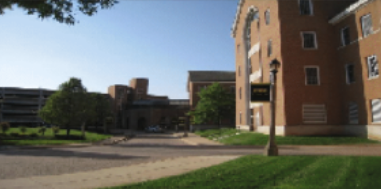
\includegraphics[width=\smallimg]{fig/seg/1/img.png}&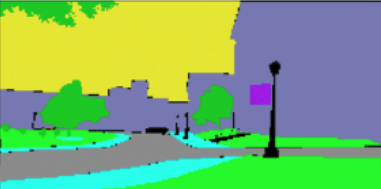
\includegraphics[width=\smallimg]{fig/seg/1/gt.png}&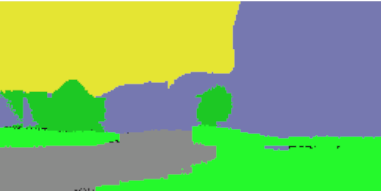
\includegraphics[width=\smallimg]{fig/seg/1/ours.png}&
\includegraphics[width=\smallimg]{fig/seg/1/glatex.png}\\

\includegraphics[width=\smallimg]{fig/seg/2/img.png}&
\includegraphics[width=\smallimg]{fig/seg/2/gt.png}&
\includegraphics[width=\smallimg]{fig/seg/2/ours.png}&
\includegraphics[width=\smallimg]{fig/seg/2/glatex.png}\\

\includegraphics[width=\smallimg]{fig/seg/3/img.png}&
\includegraphics[width=\smallimg]{fig/seg/3/gt.png}&
\includegraphics[width=\smallimg]{fig/seg/3/ours.png}&
\includegraphics[width=\smallimg]{fig/seg/3/glatex.png}\\

\includegraphics[width=\smallimg]{fig/seg/4/img.png}&
\includegraphics[width=\smallimg]{fig/seg/4/gt.png}&
\includegraphics[width=\smallimg]{fig/seg/4/ours.png}&
\includegraphics[width=\smallimg]{fig/seg/4/glatex.png}\\
\end{tabular}
\end{sc}
\end{small}
\end{center}
\vskip -0.1in
\caption{\textbf{Segmentation quality for ADE20K:} Semantic segmentation results of our method compared with GlAtEx~\protect\cite{seifi2021glimpse} on the ADE20k dataset. Qualitatively, segmentation maps produced by our method are at least as good as those of the competition.}
\label{fig:qualiative-seg}
\end{figure}

Consistently, our method obtains better results in the segmentation task than compared, state of the art methods. As presented in Table~\ref{tab:segmentation}, our approach achieves higher PA scores than those reported in~\cite{seifi2020segment} and~\cite{seifi2021glimpse}. Note, that the authors of both baseline methods present their results as mean pixel accuracy (mPA - averaged over classes), while in fact they report pixel accuracy (PA - averaged over all pixels). We confirmed this finding with the authors directly. The qualitative results presented in Figure~\ref{fig:qualiative-seg} further validate the superior performance.

\subsection{Glimpse Analysis}

\paragraph{Number of glimpses.} \begin{figure}[t]
\begin{center}
\begin{small}
\begin{sc}
\begin{subfigure}[b]{.23\textwidth}
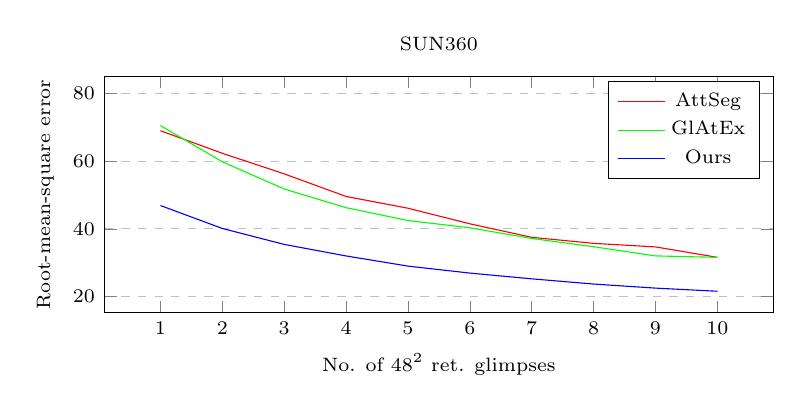
\begin{tikzpicture}
\tikzstyle{every node}=[font=\scriptsize]
\begin{axis}[
    title={SUN360},
    xlabel={No. of $48^2$ ret. glimpses},
    ylabel={Root-mean-square error},
    xtick={1,2,3,4,5,6,7,8,9,10},
    ymajorgrids=true,
    grid style=dashed,
    scale only axis,
    height=3cm,
    ymax=85,
    width=.7\textwidth
]
\addplot[color=red]
    coordinates {
    (1,68.99)(2,62.32)(3,56.24)(4,49.57)(5,46.09)(6,41.49)(7,37.49)(8,35.71)(9,34.66)(10,31.58)
    };
\addlegendentry{AttSeg}
\addplot[color=green]
    coordinates {
    (1,70.50)(2,59.81)(3,51.77)(4,46.25)(5,42.45)(6,40.31)(7,37.16)(8,34.72)(9,32.00)(10,31.58)
    };
\addlegendentry{GlAtEx}
\addplot[color=blue]
    coordinates {
    (1,46.89)(2,40.11)(3,35.40)(4,31.99)(5,28.99)(6,26.93)(7,25.23)(8,23.69)(9,22.49)(10,21.56)
    };
\addlegendentry{Ours}
\end{axis}
\end{tikzpicture}
\end{subfigure}
\begin{subfigure}[b]{.23\textwidth}
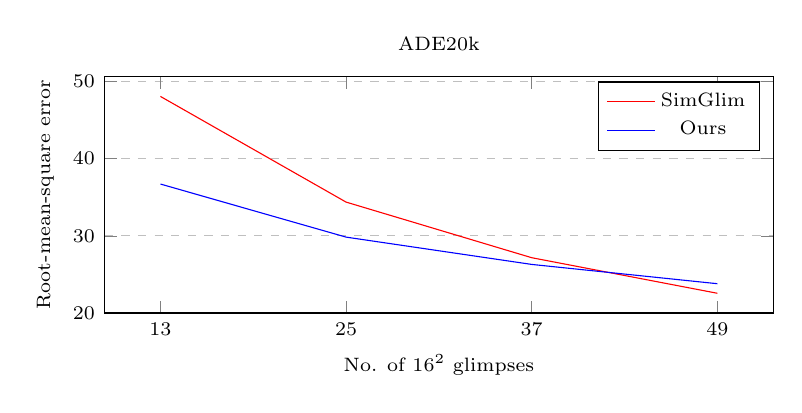
\begin{tikzpicture}
\tikzstyle{every node}=[font=\scriptsize]
\begin{axis}[
    title={ADE20k},
    xlabel={No. of $16^2$ glimpses},
    ylabel={Root-mean-square error},
    xtick={13,25,37,49},
    ymajorgrids=true,
    grid style=dashed,
    scale only axis,
    height=3cm,
    width=.7\textwidth
]
\addplot[color=red]
    coordinates {
    (13,48.08)(25,34.38)(37,27.17)(49,22.56)
    };
\addlegendentry{SimGlim}
\addplot[color=blue]
    coordinates {
    (13,36.72)(25,29.84)(37,26.30)(49,23.80)
    };
\addlegendentry{Ours}
\end{axis}
\end{tikzpicture}
\end{subfigure}
\end{sc}
\end{small}
\end{center}

\caption{\textbf{Comparative reconstruction results in regards to glimpse selection step}: Figures present the effect of the number of glimpses on the reconstruction task. On the left, we compare our model against AttSeg~\protect\cite{seifi2020segment} and GlAtEx~\protect\cite{seifi2021glimpse} on the SUN360 dataset in $48^2$ retinal glimpse scenario. On the right, we compare our model against SimGlim~\protect\cite{Jha2023WACV} on ADE20K dataset in $16^2$ non-retinal glimpse task. Our solution outperforms competitive solutions when only a small amount of the image is available.}
\label{fig:nglimpses}
\end{figure}

The relationship between model performance in the reconstruction task and the number of allowed glimpses is illustrated in Figure~\ref{fig:nglimpses}. Our model consistently outperforms all convolutional baselines. In the case of MAE-based SimGlim \cite{Jha2023WACV}, our solution performs better until around 20\% of patches are visited. This can be attributed to the fact that our solution optimizes the general reconstruction task, whereas the latter focuses on specific types of visited data when there is enough visual information already acquired.

\paragraph{Average glimpse selection.}

\begin{figure}[t]
\begin{center}
\begin{small}
\begin{sc}
\begin{tabular}{rc@{\hskip5pt}c}
Image resolution & $256\times128$ & $224\times224$ \\
Glimpse regime & $8\times48^2$ & $37\times16^2$ \\
SUN360 & \tabfigure{width=2cm}{fig/avg_glimpse/sun360.jpg} & \tabfigure{width=1cm}{fig/avg_glimpse/sun36037.jpg} \\[15pt]
ADE20k & \tabfigure{width=2cm}{fig/avg_glimpse/ade20k.jpg} &\tabfigure{width=1cm}{fig/avg_glimpse/ade20k37.jpg} 

\end{tabular}
\end{sc}
\end{small}
\end{center}
\vskip -0.1in
\caption{\textbf{Average glimpse image:} Mean glimpse map, averaged over all glimpse positions in all test images for reconstruction task on SUN360 and ADE20K. We can see that the first glimpse is consistently selected in the same place. Dataset and training regimes determine its best starting position.}
\label{fig:avg-glimpse}
\end{figure}

The average glimpse location masks are shown in Figure~\ref{fig:avg-glimpse}. For the $8\times48^2$ glimpse setup, it can be observed that the glimpse selector prefers locations in the image corners and in the center. It rarely selects locations on the left and right edge for the SUN360 dataset, which may be because the dataset consists of $360^{\circ}$ panoramic images. Selection masks for the $37\times16^2$ setup are much more evenly distributed, with only the first glimpse location being distinctive.

\subsection{Glimpse Selection Strategies}
\label{section:glimpse_selection_strategies}

\begin{table}[t]
\begin{center}
\begin{small}
\begin{sc}
\begin{tabular}{llrr}
\toprule
Selection & glimpse regime & SUN360 & MS COCO \\
\midrule
Random & $8 \times 32^2$ & 32.8 & 38.3 \\
Checker & $8 \times 32^2$ & 32.0 & 32.6 \\
Attention & $8 \times 32^2$ & \textbf{29.8} & \textbf{32.5} \\
\midrule
Random & $8 \times 16^2$ & 39.8 & 47.3\\
Checker & $8 \times 16^2$ & 39.3 & 44.1 \\
Attention & $8 \times 16^2$ & \textbf{37.9} & \textbf{43.2} \\
\bottomrule
\end{tabular}
\end{sc}
\end{small}
\end{center}
\vskip -0.1in
\caption{\textbf{AME-based glimpse selection versus naive sampling - reconstruction:} Comparison of glimpse selection strategies for reconstruction task on SUN360 and MS COCO databases. The metric used is a root mean square error (RMSE; lower is better). We used regular (non-retinal) glimpses for this ablation. Our method performs better than random position sampling and random sampling from a checkerboard-like pattern.}
\label{tab:selection-reconstruction}
\end{table}
\begin{table}[t]
\begin{center}
\begin{small}
\begin{sc}
\begin{tabular}{llrr}
\toprule
Selection & glimpse regime & train all & head-only \\
\midrule
Random & $8 \times 32^2$ & 72.4	& 66.2 \\
Checker & $8 \times 32^2$ & 70.1 &64.0 \\
Attention & $8 \times 32^2$ & \textbf{73.4} & \textbf{66.9} \\
\midrule
Random & $8 \times 16^2$ & 61.9	& 53.7\\
Checker & $8 \times 16^2$ & 57.8 & \textbf{56.2} \\
Attention & $8 \times 16^2$ & \textbf{63.4} & 55.9 \\
\bottomrule
\end{tabular}
\end{sc}
\end{small}
\end{center}
\vskip -0.1in
\caption{\textbf{AME-based glimpse selection versus naive sampling - classification:} Comparison of glimpse selection strategies in classification task for SUN360 database. The metric used is accuracy (higher is better). We used regular (non-retinal) glimpses for this ablation and tested full-model and head-only training strategies. Our method performs better than random position sampling and random sampling from a checkerboard-like pattern.}
\label{tab:selection-classification}
\end{table}

Our attention-based glimpse selection process outperforms random glimpse selection and a fixed checkerboard-like glimpse pattern, as demonstrated in Table~\ref{tab:selection-reconstruction} and \ref{tab:selection-classification}. This supports our claim that our selection strategy is superior to naive strategies and contradicts the discussions presented in \cite{Jha2023WACV}.

\paragraph{Level of attention map.}

\begin{figure}[t]
\begin{center}
\begin{small}
\begin{sc}

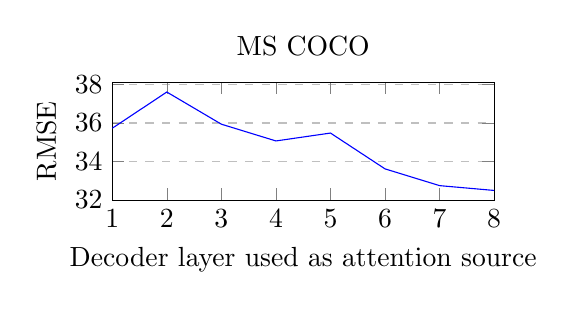
\begin{tikzpicture}
\begin{axis}[
    title={MS COCO},
    xlabel={Decoder layer used as attention source},
    ylabel={RMSE},
    xtick={1,2,3,4,5,6,7,8},
    xmin=1,
    xmax=8,
    ymajorgrids=true,
    grid style=dashed,
    scale only axis,
    height=1.5cm,
    width=.4\textwidth
]
\addplot[color=blue]
    coordinates {
    (1,35.73)(2,37.61)(3,35.94)(4,35.07)(5,35.48)(6,33.62)(7,32.75)(8,32.5)
    };
\end{axis}
\end{tikzpicture}
\end{sc}
\end{small}
\end{center}

\caption{\textbf{RMSE results versus attention map source:} Comparison of attention-based glimpse selection results in regards to decoder layer used as attention map source. The figure shows that the best results can be achieved using the last layer of the decoder. The dataset used is MS COCO. The metric is a root mean square error (RMSE; lower is better). The image resolution is $256\times128$ in an $8\times32^2$ non-retinal glimpse regime.}
\label{fig:attention-layer}
\end{figure}

In Figure \ref{fig:attention-layer}, we demonstrate the impact of the choice of decoder layer as the attention map source on the model performance. The results show that the further in the decoder the attention maps are sourced from, the better the overall performance.

\section{Conclusions}

This paper presents a new approach to active visual exploration that simplifies the existing methods by leveraging internal model uncertainty in glimpse selection process. By utilizing the entropy of the transformer's attention maps, we eliminate the need for any sampling decision module or separate network head focused on decision strategy. Furthermore, our approach does not require separate training for the main task and the sampling decision strategy, reducing the complexity of the overall system. Our approach is based on the masked auto-encoder architecture, which allows for the efficient processing of partial observations. The results demonstrate that the attention values trained inherently from the transformer-based decoder can be used to generate decision-making priors that improve the performance of scene understanding tasks. An exhaustive empirical comparison against the competing architectures shows that our solution performs better when limited data is available.

% We also identify the limitations of our approach in the segmentation task. The performance of our method, being transformer-based, is hindered when coupled with the low resolution data and small number of available patches. Hence, we acknowledge that our method inherits some of the limitations of contemporary transformer architectures, and identify that further work on its robustness is needed.% future work thus there is room for further development in this area.


\appendix


\section*{Acknowledgments}

This research was funded by National Science Centre, Poland (grants no 2020/39/B/ST6/01511, 2022/45/B/ST6/02817, and 2021/41/B/ST6/01370), Foundation for Polish Science (grant no POIR.04.04.00-00-14DE/18-00 carried out within the Team-Net program co-financed by the European Union under the European Regional Development Fund). We gratefully acknowledge Polish high-performance computing infrastructure PLGrid (HPC Centers: ACK Cyfronet AGH) for providing computer facilities and support within computational grant no. PLG/2022/015753. The research was supported by a grant from the Faculty of Mathematics and Computer Science under the Strategic Programme Excellence Initiative at Jagiellonian University.

%% The file named.bst is a bibliography style file for BibTeX 0.99c
\bibliographystyle{named}
\bibliography{example_paper}

\end{document}


              
              
              
              
              
              
              
              
              
              
              
              
              
              
              
              
          

              
              
              
              
              
              
              
              
              
              
              
              
              
              
              
              
          

              
              
              
              
              
              
              
              
              
              
              
              
              
              
              
              
          

              
              
              
              
              
              
              
              
              
              
              
              
              
              
              
              
          

              
              
              
              
              
              
              
              
              
              
              
              
              
              
              
              
          